% article example for classicthesis.sty
\documentclass[10pt,a4paper]{article} % KOMA-Script article scrartcl
\usepackage{import}
\usepackage{xifthen}
\usepackage{pdfpages}
\usepackage{transparent}
\newcommand{\incfig}[1]{%
    \def\svgwidth{\columnwidth}
    \import{./figures/}{#1.pdf_tex}
}
\usepackage{lipsum}     %lorem ipsum text
\usepackage{titlesec}   %Section settings
\usepackage{titling}    %Title settings
\usepackage[margin=10em]{geometry}  %Adjusting margins
\usepackage{setspace}
\usepackage{listings}
\usepackage{amsmath}    %Display equations options
\usepackage{amssymb}    %More symbols
\usepackage{xcolor}     %Color settings
\usepackage{pagecolor}
\usepackage{mdframed}
\usepackage[spanish]{babel}
\usepackage[utf8]{inputenc}
\usepackage{longtable}
\usepackage{multicol}
\usepackage{graphicx}
\graphicspath{ {./Images/} }
\setlength{\columnsep}{1cm}

% ====| color de la pagina y del fondo |==== %
\pagecolor{black}
\color{white}



\begin{document}
    %========================{TITLE}====================%
    \title{{  Notas Tema 2 AED  }}
    \author{{Rodrigo Castillo}}
    \date{\today}

    \maketitle


     % ====| Loguito |==== %
    
\includegraphics[width=0.1\linewidth]{negro_cara.png}
    %=======================NOTES GOES HERE===================%
    \section{Distancia Euclideana}
        \begin{itemize}
            \item {la mayoria de las tecnicas multivariables dependen del
                concepto de distancia}
        \end{itemize}
        sean $ P = (x_1 , x_2 , x_3 ... , x_p)  $ y $ Q = (y_1 , y_2 , y_3 , ... , y_p)  $ se tiene que la distancia entre P y Q está dada como  :
        \begin{equation}
            \color{red} d(P,Q) = \sqrt{(x_1 - y_1) ^{2} + (x_2 - y_2)^{2} + ...
            + (x_p - y_p) ^{2}   }  \color{white}
        \end{equation}
        \begin{itemize}
            \item {la distancia euclideana sirve para medir distancias entre 2
                puntos pero en estadística no sirve, se usa una distancia
            llamada Distancia Estadística}
            \item {no funciona porque cada coordenada pesa lo mismo }
            \item {en la estadistica es bueno darle mayor peso a las variables
                que varian menos y menor peso a aquellas que varian mas}
            \item {la distancia estadístca tiene en cuenta tanto el peso de la variacion como el peso de las variables}
        \end{itemize}
    \section{Distancia Estadistica}
        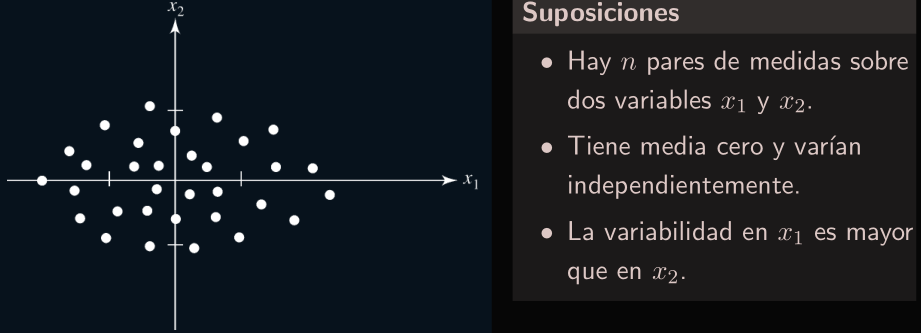
\includegraphics[width=0.8\linewidth]{dis.png}
        \begin{itemize}
            \item {los puntos respecto al origen en la direccion de $ x_1  $
                son mas comunes que los puntos a la misma distancia en la
            dirección $ x_2  $ }
            \item {por lo tanto la variabilidad de $ x_1   $ es mayor que la de
                $ x_2  $  }
            \item {son mas comunes coordenadas grandes en $ x_1  $ que en $ x_2
                $  }
            \item {tiene sentido ponderar mas a $ x_2  $ que a $ x_1  $ }
        \end{itemize}
        para construir la distancia estadística ...
        \begin{enumerate}
            \item {$ x_1 ^{*} = \frac{x}{\sqrt{s_{11}}  }  $  y $ x_2 ^{*}  =
                    \frac{x_2}{\sqrt{S_{22}} }$  para ponderar las coordenadas con menor variabilidad }
                \item {aplicamos la distancia euclideana para definir la
                    distancia entre el punto $ P=(x_1 , x_2 )  $ al origen $ O
                = (0,0)  $ }
                \item {si la variabilidad de ambas distancias es igual, se usa
                    la distancia euclideana}
        \end{enumerate}
        \begin{figure}[h!]
            \centering
            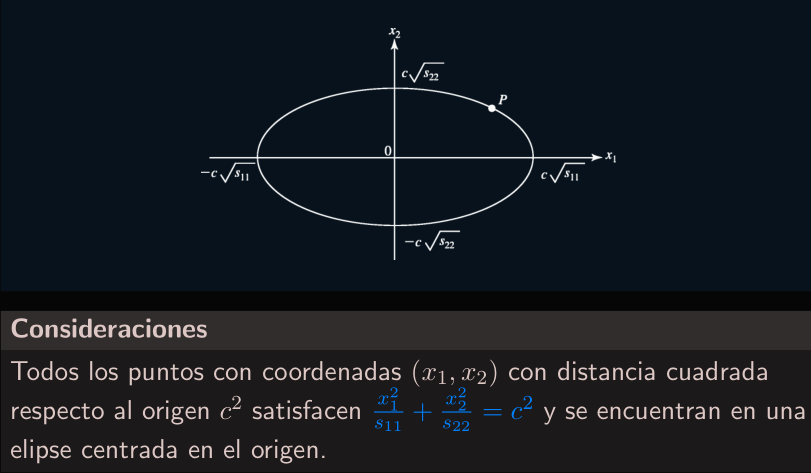
\includegraphics[width=0.8\linewidth]{consideraciones.png}
            \caption{Consideraciones}
            \label{fig:consideraciones}
        \end{figure}
        por lo tanto la distancia estadística está dada como :
        \begin{equation}
            \color{red}D_{estadistica}(P,Q) = \sqrt{ \frac{(x_1 - y_1)}{s_{11}} ^{2} +
            \frac{(x_2 -
            y_2)}{s_{22}} ^{2} + ... + \frac{x_{pp}- y_p }{s_{pp}} ^{2} }
            \color{white}
        \end{equation}
        \begin{itemize}
            \item {todos los puntos $ P  $ están a una distancia cuadrada
                constante del punto $ Q  $ yacen sobre una hiper elipsoide
            centrada en $ Q  $  con ejes mayor y menor paralelos a los ejes
            coordenados}
            \item {la distancia desde $ P  $ hasta el origen $ O  $ se puede
                obtener mediante $ y_1 = y_2 = y_3 ... y_p = 0  $ }
            \item {si $ s_{11} = s_{22}   $ da igual que usar la distancia
                euclideana}
            \item {la distancia estadistica supone que las coordenadas son
                independientes}
            \item {no incluye los casos importantes}

        \newpage
        \end{itemize}
        \begin{figure}[h!]
            \centering
            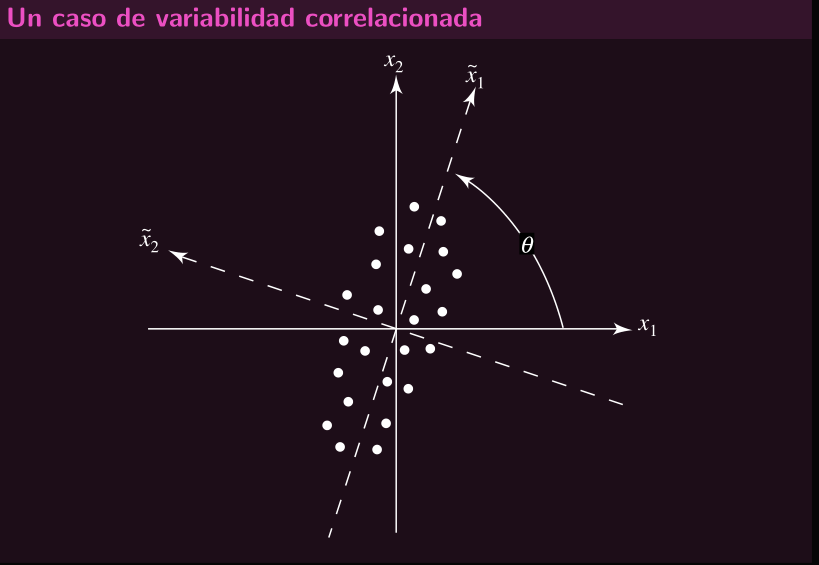
\includegraphics[width=0.8\linewidth]{caso.png}
            \caption{Caso}
            \label{fig:caso}

        \end{figure}
        \begin{figure}[h!]
            \centering
            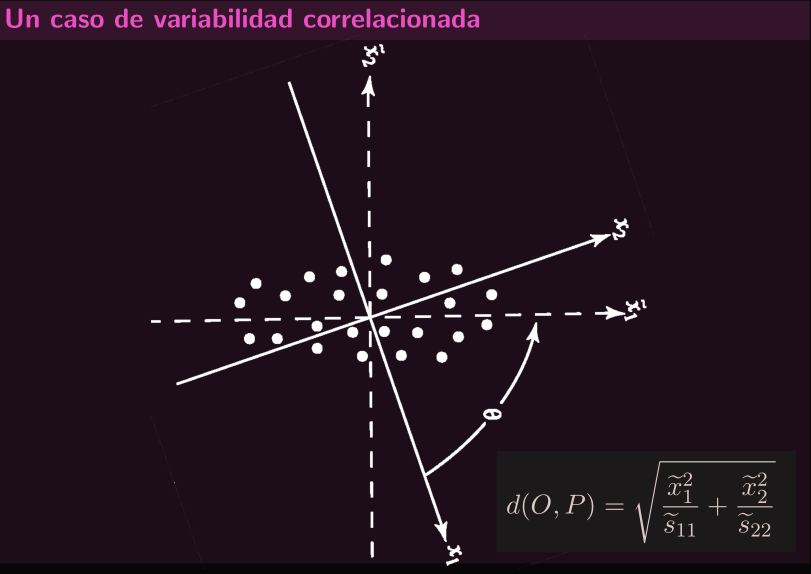
\includegraphics[width=0.8\linewidth]{caso2.png}
            \caption{Caso2}
            \label{fig:caso2}
        \end{figure}

        cuando las variables están correlacionadas , la variable a un punto
        \color{red} fijo \color{white} es ...
        \begin{equation}
        \color{red}     D(P,Q) = \sqrt{ a_{11}(x_1 - y_1) ^{2}  +
            2a_{12}(x_1-y_1)(x_2-y_2)
            } \color{white}
        \end{equation}
        esta distancia puede ser calculada una vez se cauclulen $ a_{11}
        ,a_{12} , a_{22}  $

        \newpage
        \begin{figure}[h!]
            \centering
            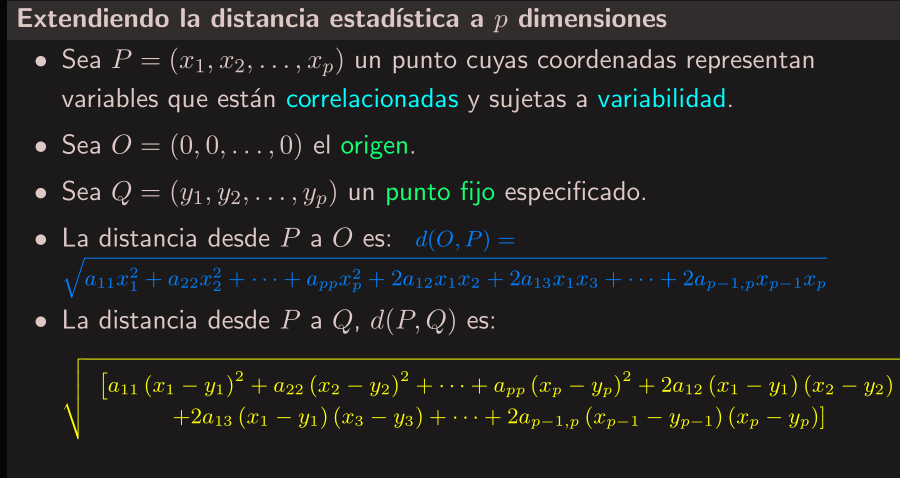
\includegraphics[width=0.8\linewidth]{pdim.png}
            \caption{P-Dimensiones}
            \label{fig:pdim}
        \end{figure}
        Ahora, de forma matricial la distancia queda como :
        \begin{figure}[h!]
            \centering
            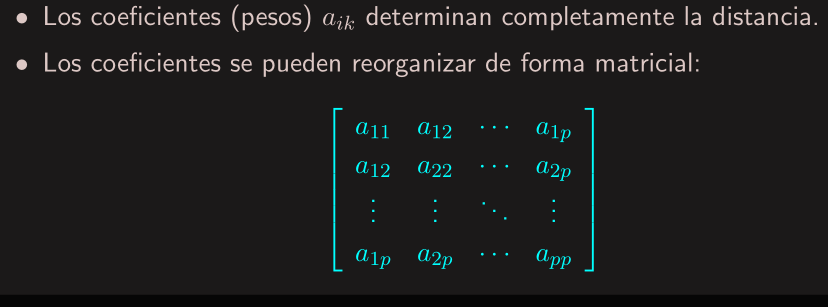
\includegraphics[width=0.5\linewidth]{matricial.png}
            \caption{Matricial}
            \label{fig:matricial}
        \end{figure}

    \section{cosas de repaso}
        producto interno
        \begin{equation}
             \color{red} x'y=x_1 y_1 + x_2 y_2 + ... + x_n y_n
             \color{white}
         \end{equation}

         longitud de un vector
         \begin{equation}
            \color{red}  L_x = \sqrt{x_1 ^{2} + x_2 ^{2} + ... + x_n ^{2}   } = \sqrt{x'x}
 \color{white}          \end{equation}
     angulo entre dos vectores ...
        \begin{equation}
            \color{red} \cos{\theta }  = \frac{x'y }{L_x L_y} = \frac{x'y}{\sqrt{x'x}
            \sqrt{y'y}  } \color{white}
        \end{equation}

    independencia lineal

    \\ un conjunto de vectores $ x_1 , x_2 , x_3 , ... , x_ n  $ si existen
    constantes $ c_1 ... c_n  $  tales que \color{red} $ x_1 c_1 + c_2 x_2 +
    ... + c_{k}x_k
    = 0    $ \color{white}
    \\
    \section{Dudas}
        \begin{enumerate}
            \item {\color{green} no me queda claro la ecuacion 2 de donde sale
                la ecuacion 3 \color{white}  }
        \end{enumerate}











    %=======================NOTES ENDS HERE===================%

    % bib stuff
    \nocite{*}
    \addtocontents{toc}{{}}
    \addcontentsline{toc}{section}{\refname}
    \bibliographystyle{plain}
    \bibliography{../Bibliography}
\end{document}
